\chapter{Experiments and Results}\label{chapter:experiments}

This chapter is dedicated to an overview of the experiments and tests made for the implemented CASA system, and their results. Here, prerecorded monophonic piano sounds from the input dataset will be listed firstly, and then each of the four following sections will describe a specific set of experiments in detail. In these sections, the reader will find conversations about the tests for input sounds mixed with white noise of different levels, or with other prerecorded sounds in the background, tests in connection with a simple classifier, and other experiments for various input parameters.

\section{Dataset Overview}\label{section:experiments_dataset}

The set of input data for testing consisted of 34 piano recordings of various scales and intervals. Each file was converted to the WAV file format to address the limitations of the employed packages. Below is a more detailed overview:

\begin{description}
	\item[A-major] scale played fast and slow in ascending and descending order, starting from $A_3$ and ending at $A_4$
	\item[A-minor] scale played fast and slow in ascending and descending order in three modes: natural, harmonic and melodic, starting from $A_3$ and ending at $A_4$
	\item[C-major] scale played fast and slow in ascending and descending order, starting from $C_4$ and ending at $C_5$
	\item[C-major] scale, where each note is repeated 3 times, in ascending order in four variants: starting from $C_3$, $C_4$, $C_5$ and $C_6$ and ending one octave higher
	\item[D-major] scale played fast and slow in ascending and descending order, starting from $D_4$ and ending at $D_5$
	\item[E-major] scale played fast and slow in ascending and descending order, starting from $E_4$ and ending at $E_5$
	\item[E-minor] scale played fast and slow in ascending and descending order in three modes: natural, harmonic and melodic, starting from $E_4$ and ending at $E_5$
	\item[F-major] scale played fast and slow in ascending and descending order, starting from $F_4$ and ending at $F_5$
	\item[G-major] scale played fast and slow in ascending and descending order, starting from $G_4$ and ending at $G_5$
	\item[H-major] scale played fast and slow in ascending and descending order, starting from $H_4$ and ending at $H_5$
	\item[Perfect melodic fourths] with lower notes in range starting from $C_3$ and ending at $C_6$, in ascending order
	\item[Perfect melodic octaves] with lower notes in range starting from $C_3$ and ending at $F_5$, in ascending order
	\item[All semitones] (or all piano keys one after another), starting from $C_4$ and ending at $H_5$, in ascending order
	\item[All semitones] (or all piano keys one after another), starting from $C_2$ and ending at $H_3$, in ascending order
\end{description}

\section{Experiments with White Noise}

The first set of experiments involved experiments with white noise levels. The white noise level was an input parameter of the CASA system, and was used before the peripheral analysis stage as an amplitude multiplier for the generated white noise wave, where samples for the digital signal were randomly picked from a normal distribution of mean 0 and variance 1. This modified wave was added to the target signal and considered the background. The example set of values was as follows: $\left\{0;~0.005;~0.01;~0.02;~0.04\right\}$, and the results for it are shown on figure \ref{img:white_noise_experiments}.\\

On the figure, the first row depicts the outcomes of processing a clean target signal (A-major scale played fast), and each next row shows the results for the added white noise levels in ascending order. When comparing the cochleagrams, the rising amounts of background interference can be clearly seen (the dark-blue color in the first cochleagram becomes brighter with each itera\-tion). From the resulting masking, it can be observed that the model began to lose the quality of source separation when the noise level was around $0.02$, which is clearly a major amount of randomness in the input, and can be well heard by a human listener. Given the simplicity of the algorithm for the segmentation-and-grouping stage, the outcomes can be considered a success.\\

As an improvement of the resulting source separation, the masks computed for clean target signals were used on cochleagrams for signals with noise. This method was inspired by the fact that human brain tends to remember sounds heard before (the word "sound" is used here in a more psychological sense), and then use this knowledge to analyze a complex auditory scene more easily. This memory-based approach, however, would not have been possible, if clean target sounds had not been known beforehand.

\begin{figure}[htp]
	\centering
	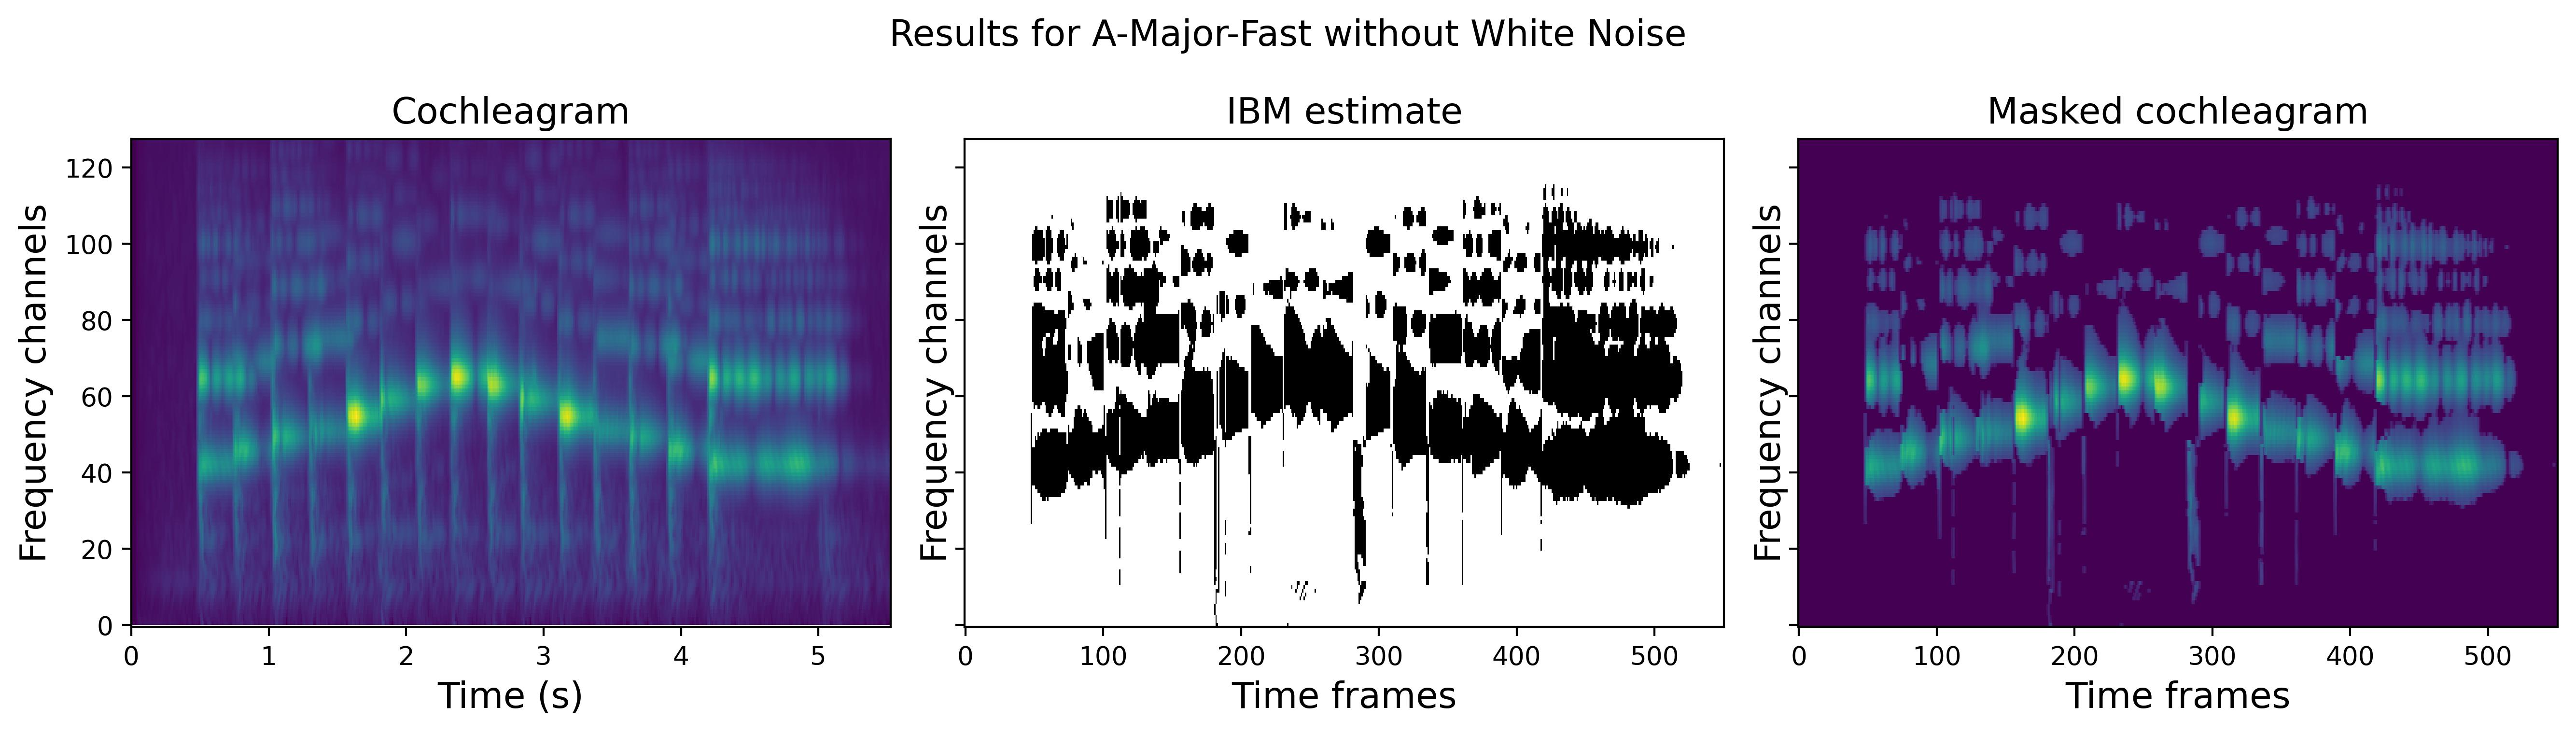
\includegraphics[width=\textwidth]{include/experiments_A-major-fast_WN_0,0.jpg}
	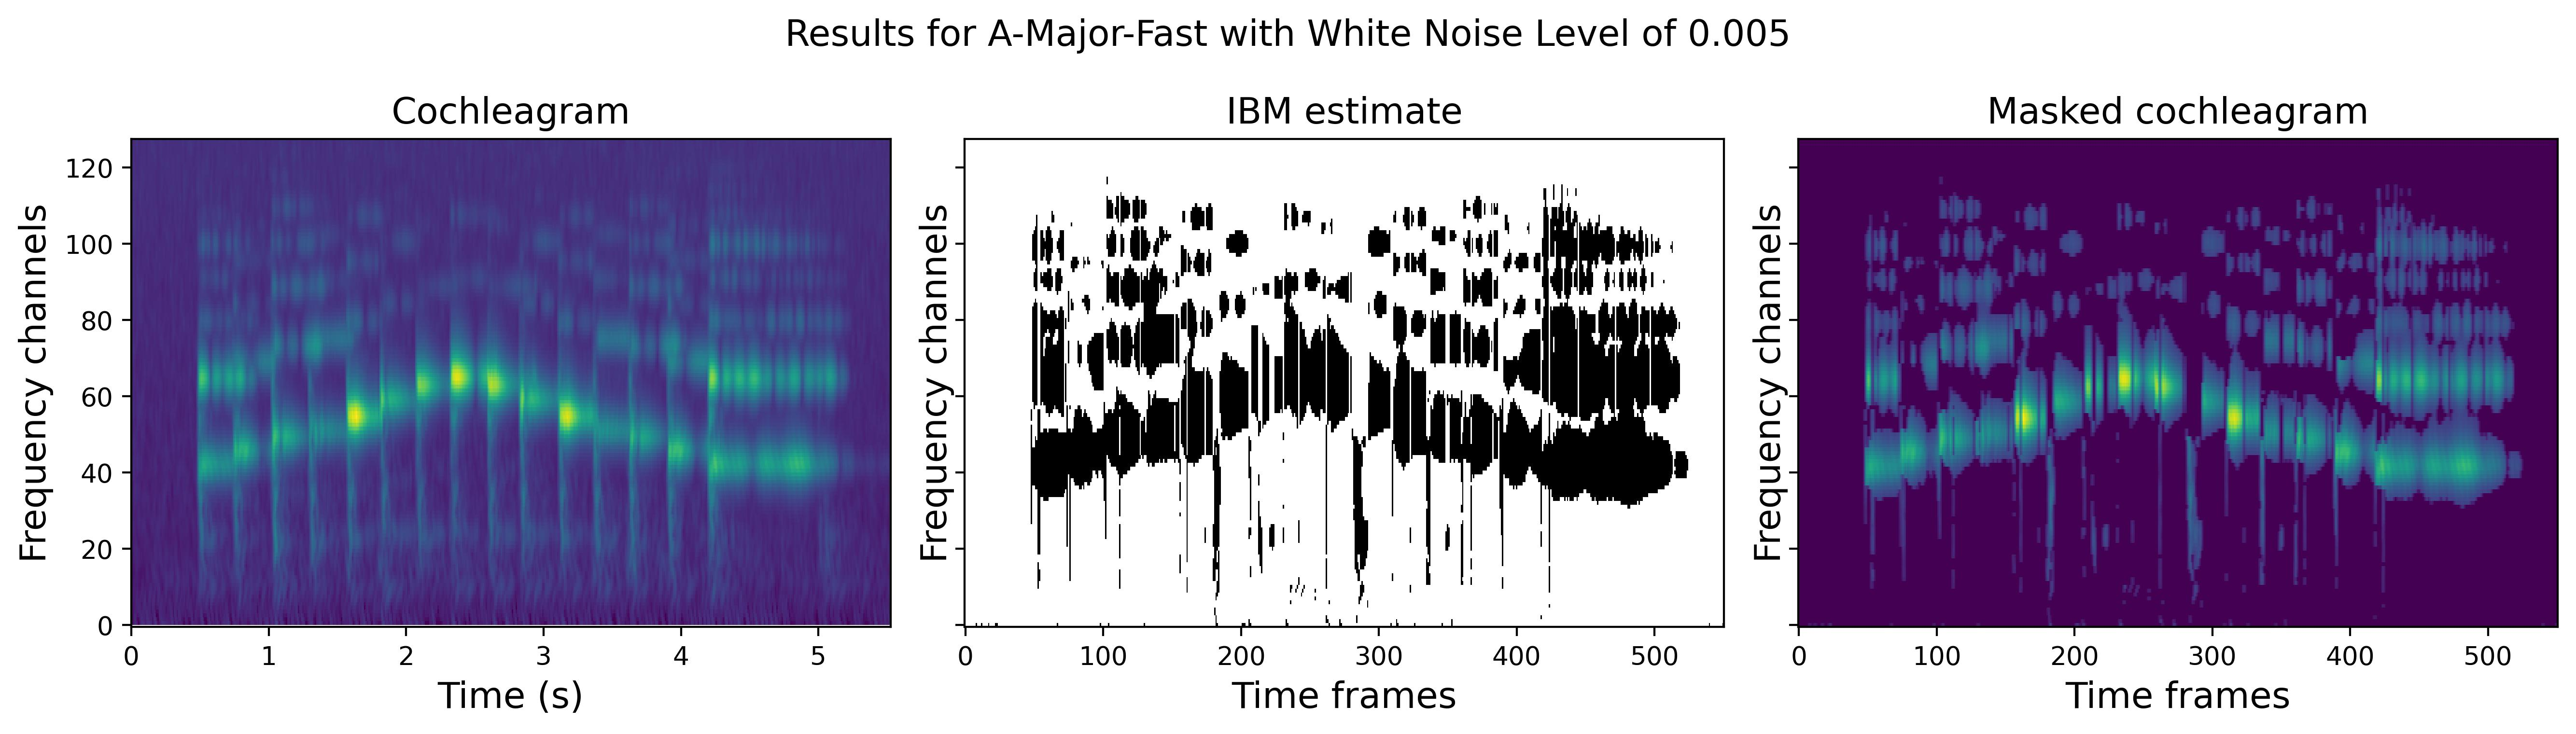
\includegraphics[width=\textwidth]{include/experiments_A-major-fast_WN_0,005.jpg}
	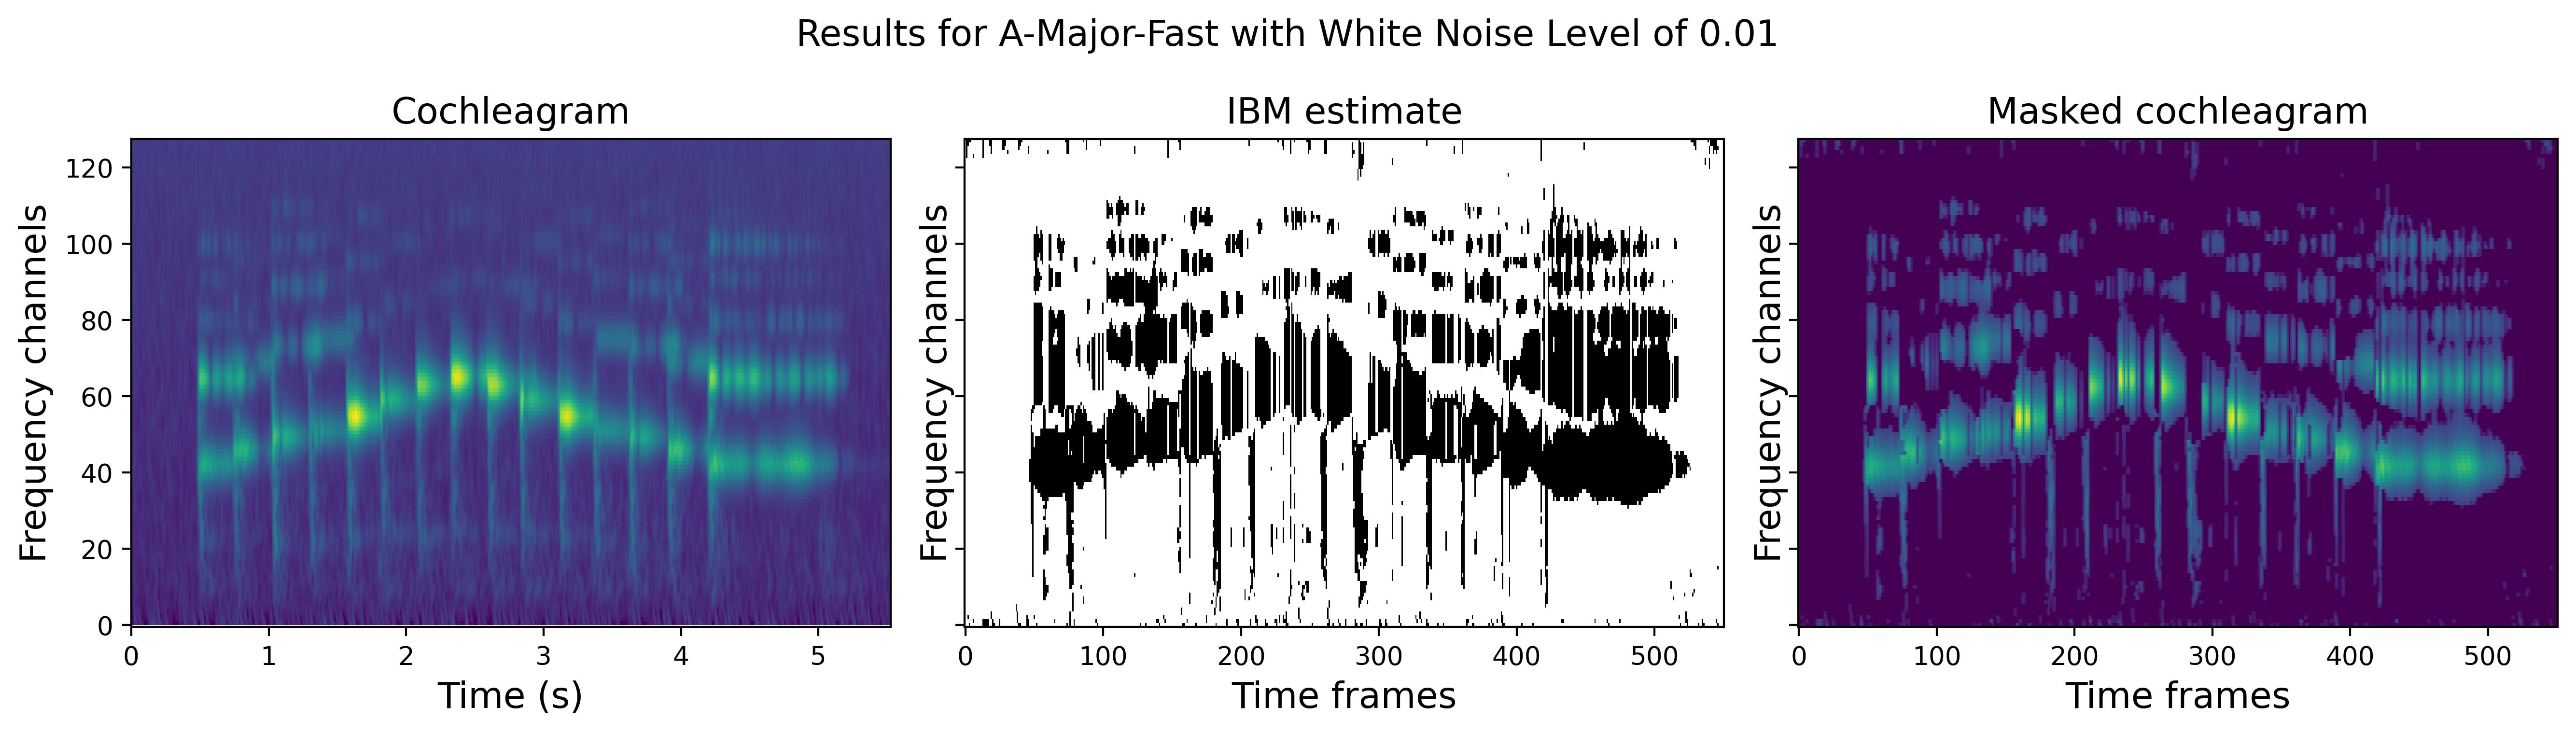
\includegraphics[width=\textwidth]{include/experiments_A-major-fast_WN_0,01.jpg}
	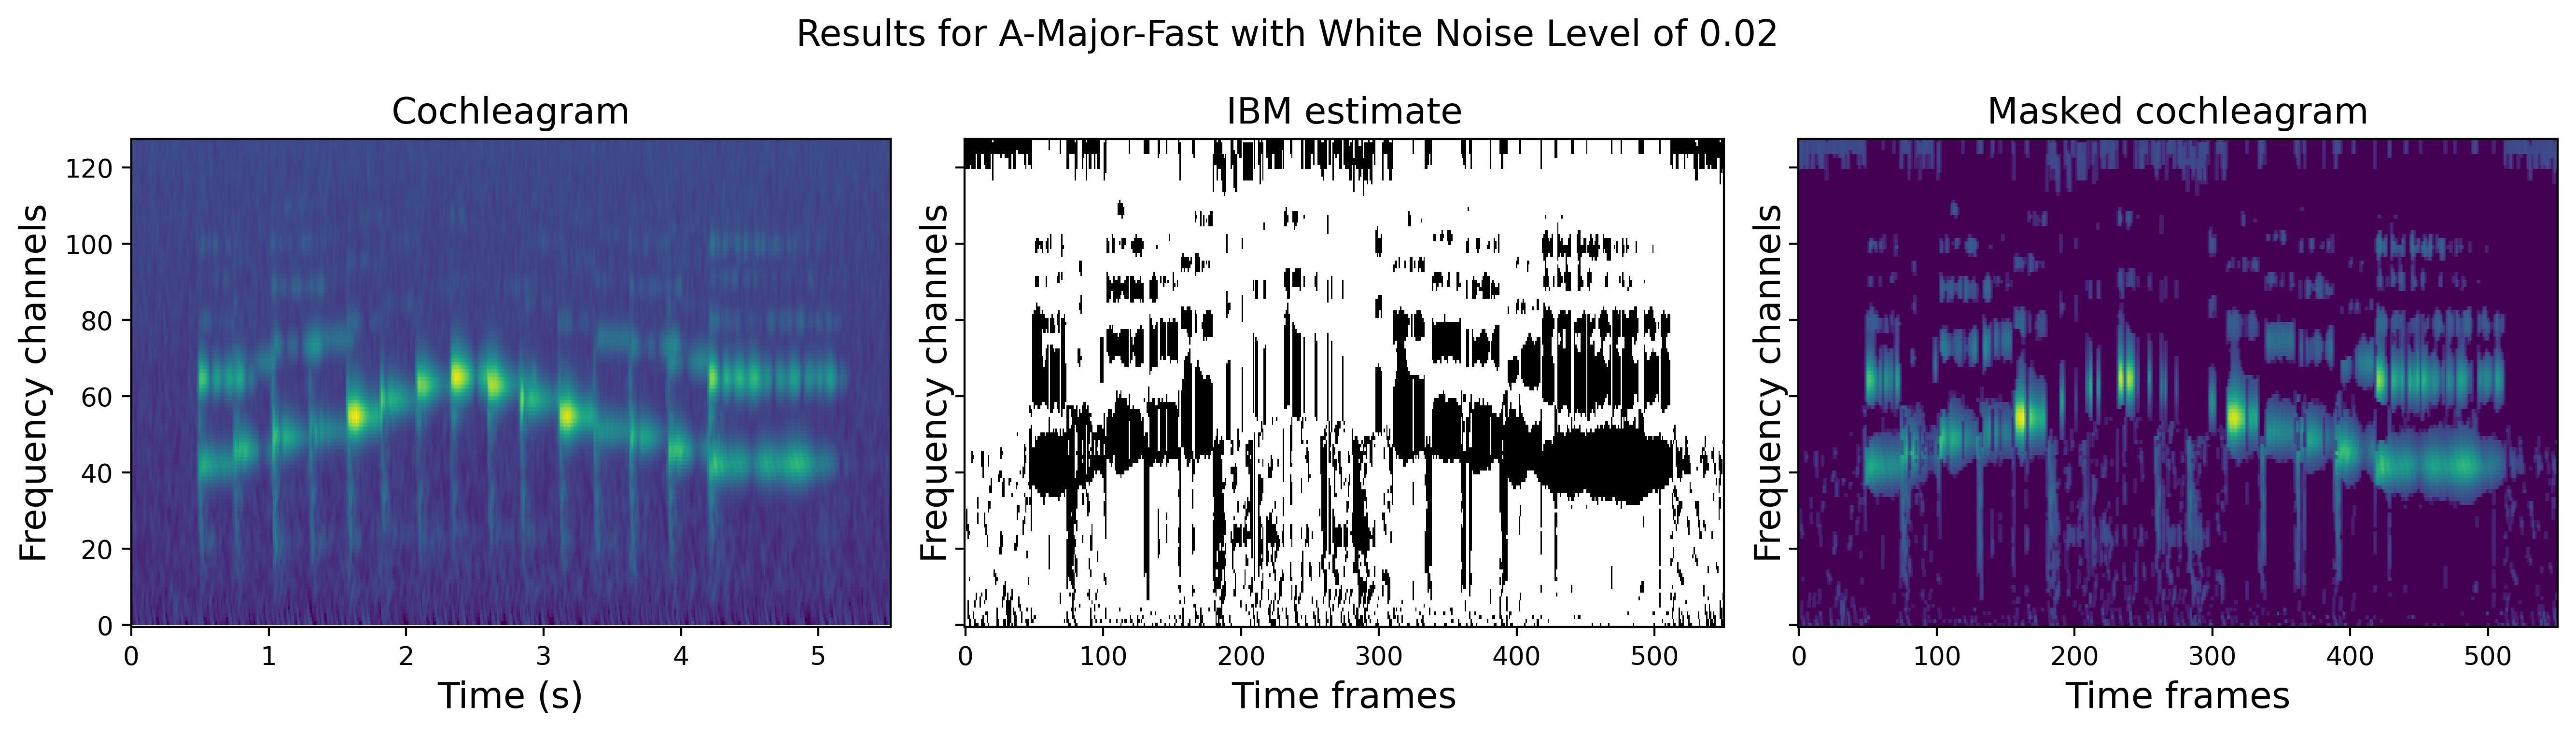
\includegraphics[width=\textwidth]{include/experiments_A-major-fast_WN_0,02.jpg}
	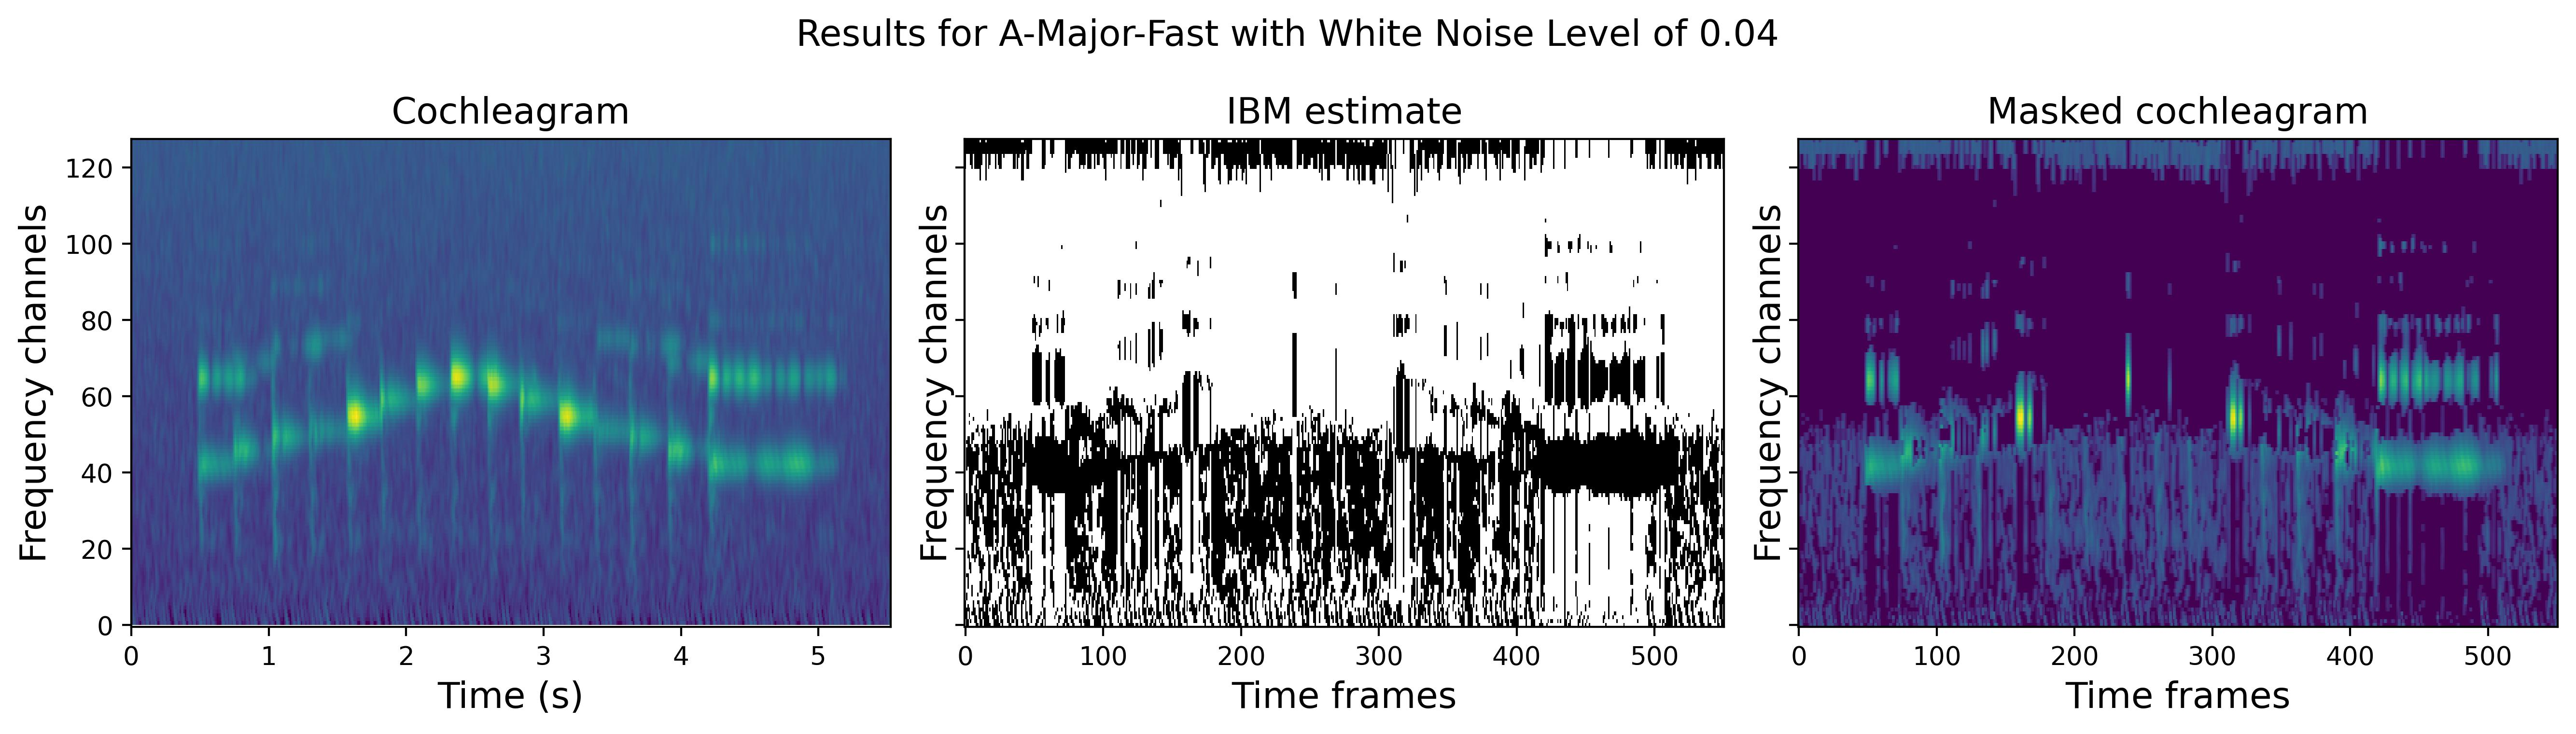
\includegraphics[width=\textwidth]{include/experiments_A-major-fast_WN_0,04.jpg}
	\caption[Results of experiments with white noise levels]{Results of the experiments with A-major scale mixed with white noise of different amplitudes. In each row, the first image is a cochleagram of the input sound, the second is the estimated IBM, and the third is the masked cochleagram.}
	\label{img:white_noise_experiments}
\end{figure}

\begin{figure}[htp]
	\centering
	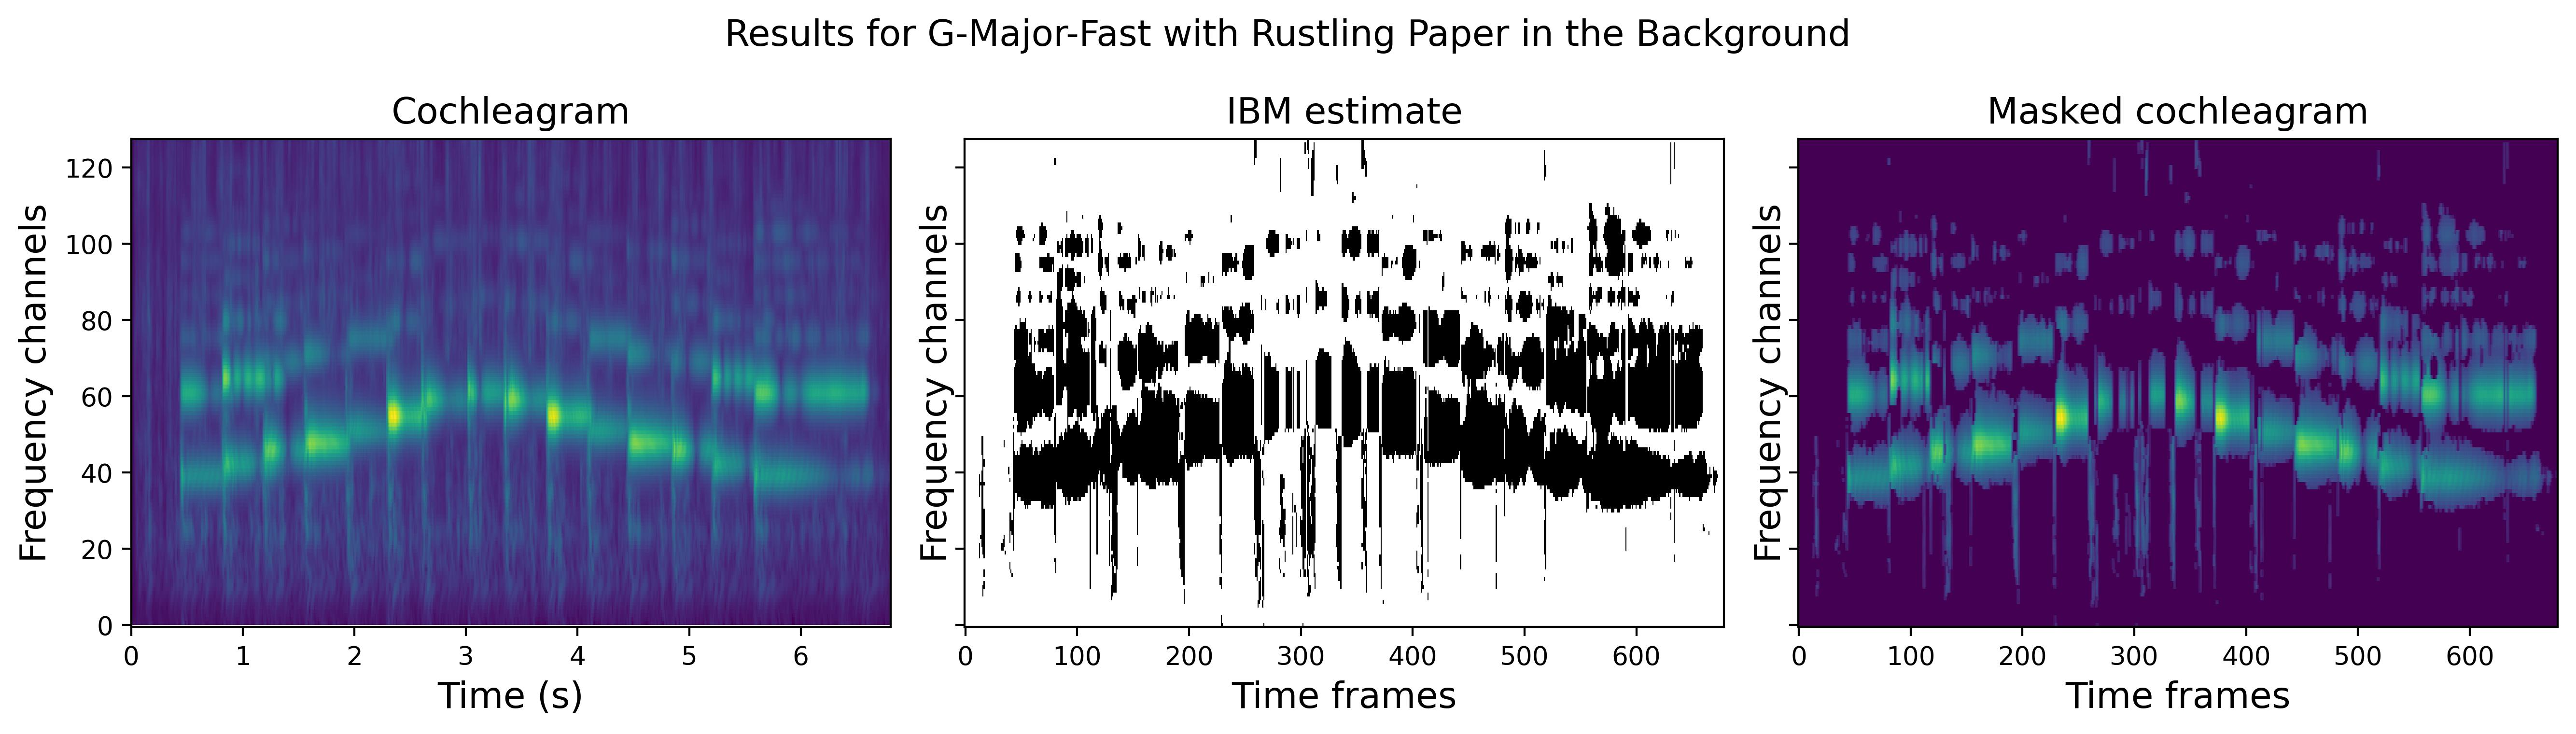
\includegraphics[width=\textwidth]{include/experiments_G-major-fast_BG2.jpg}
	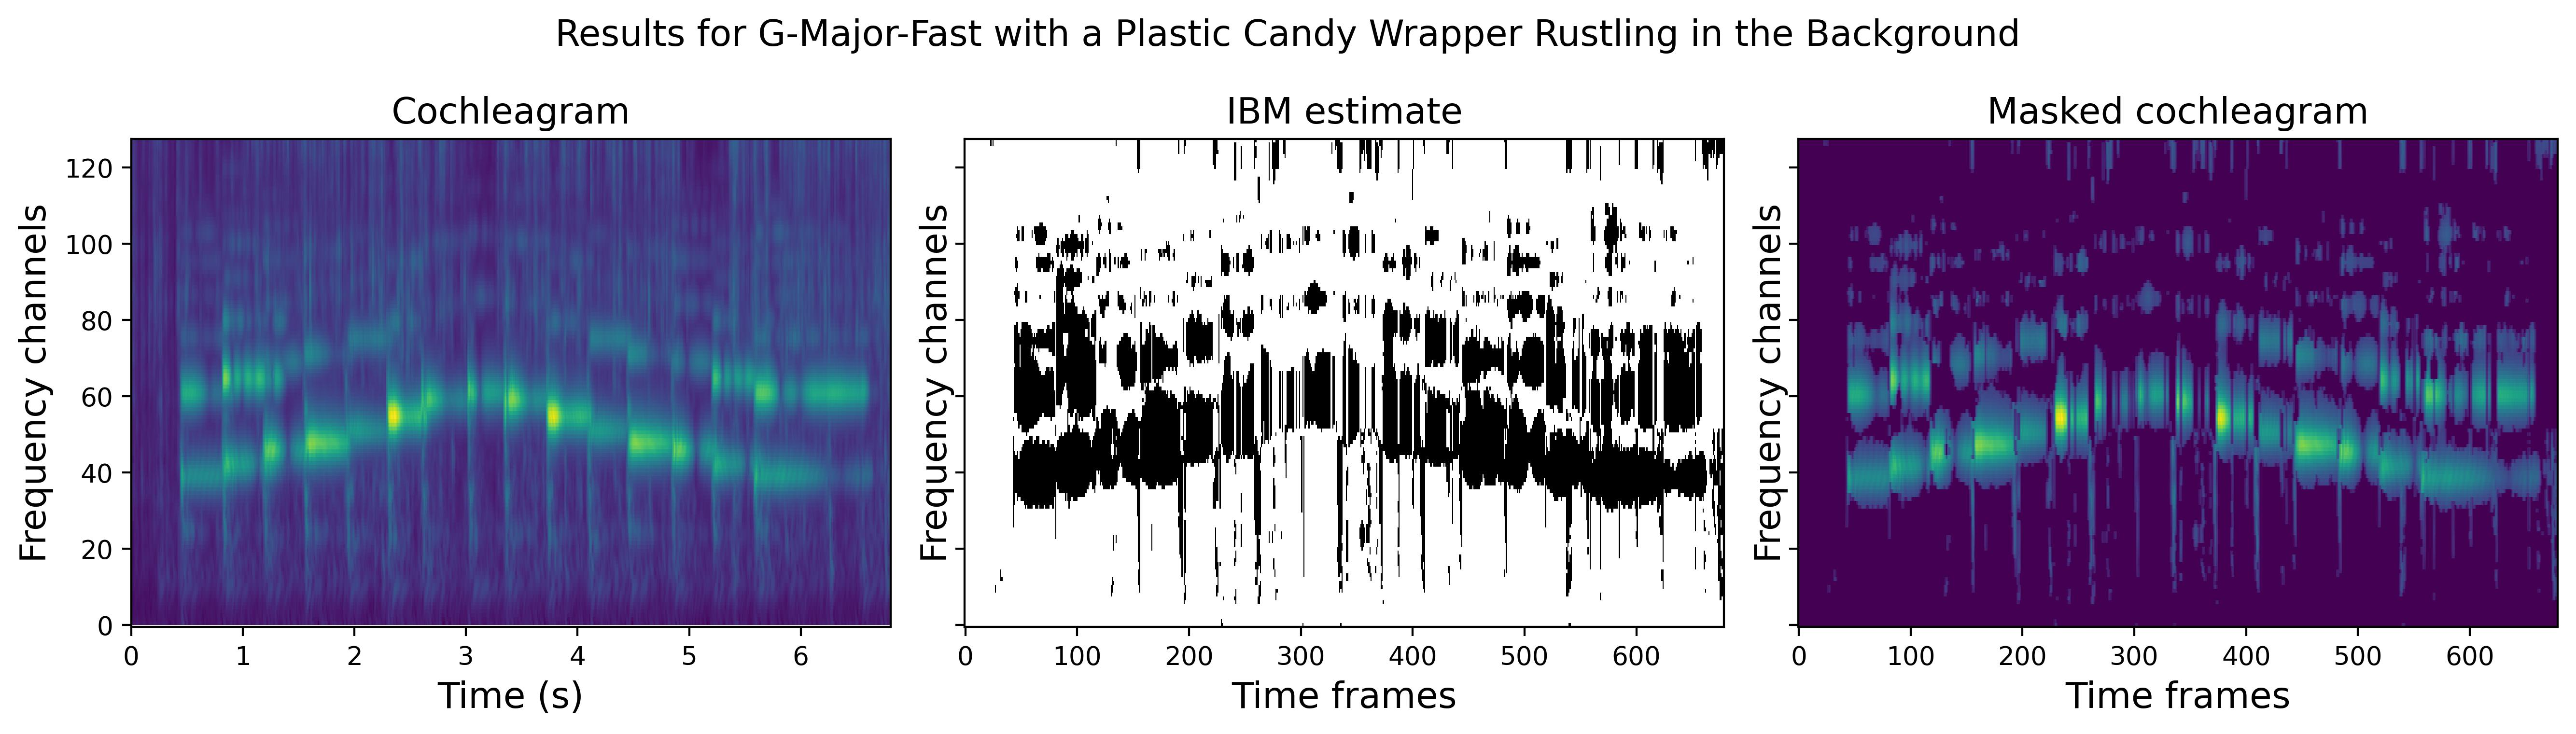
\includegraphics[width=\textwidth]{include/experiments_G-major-fast_BG3.jpg}
	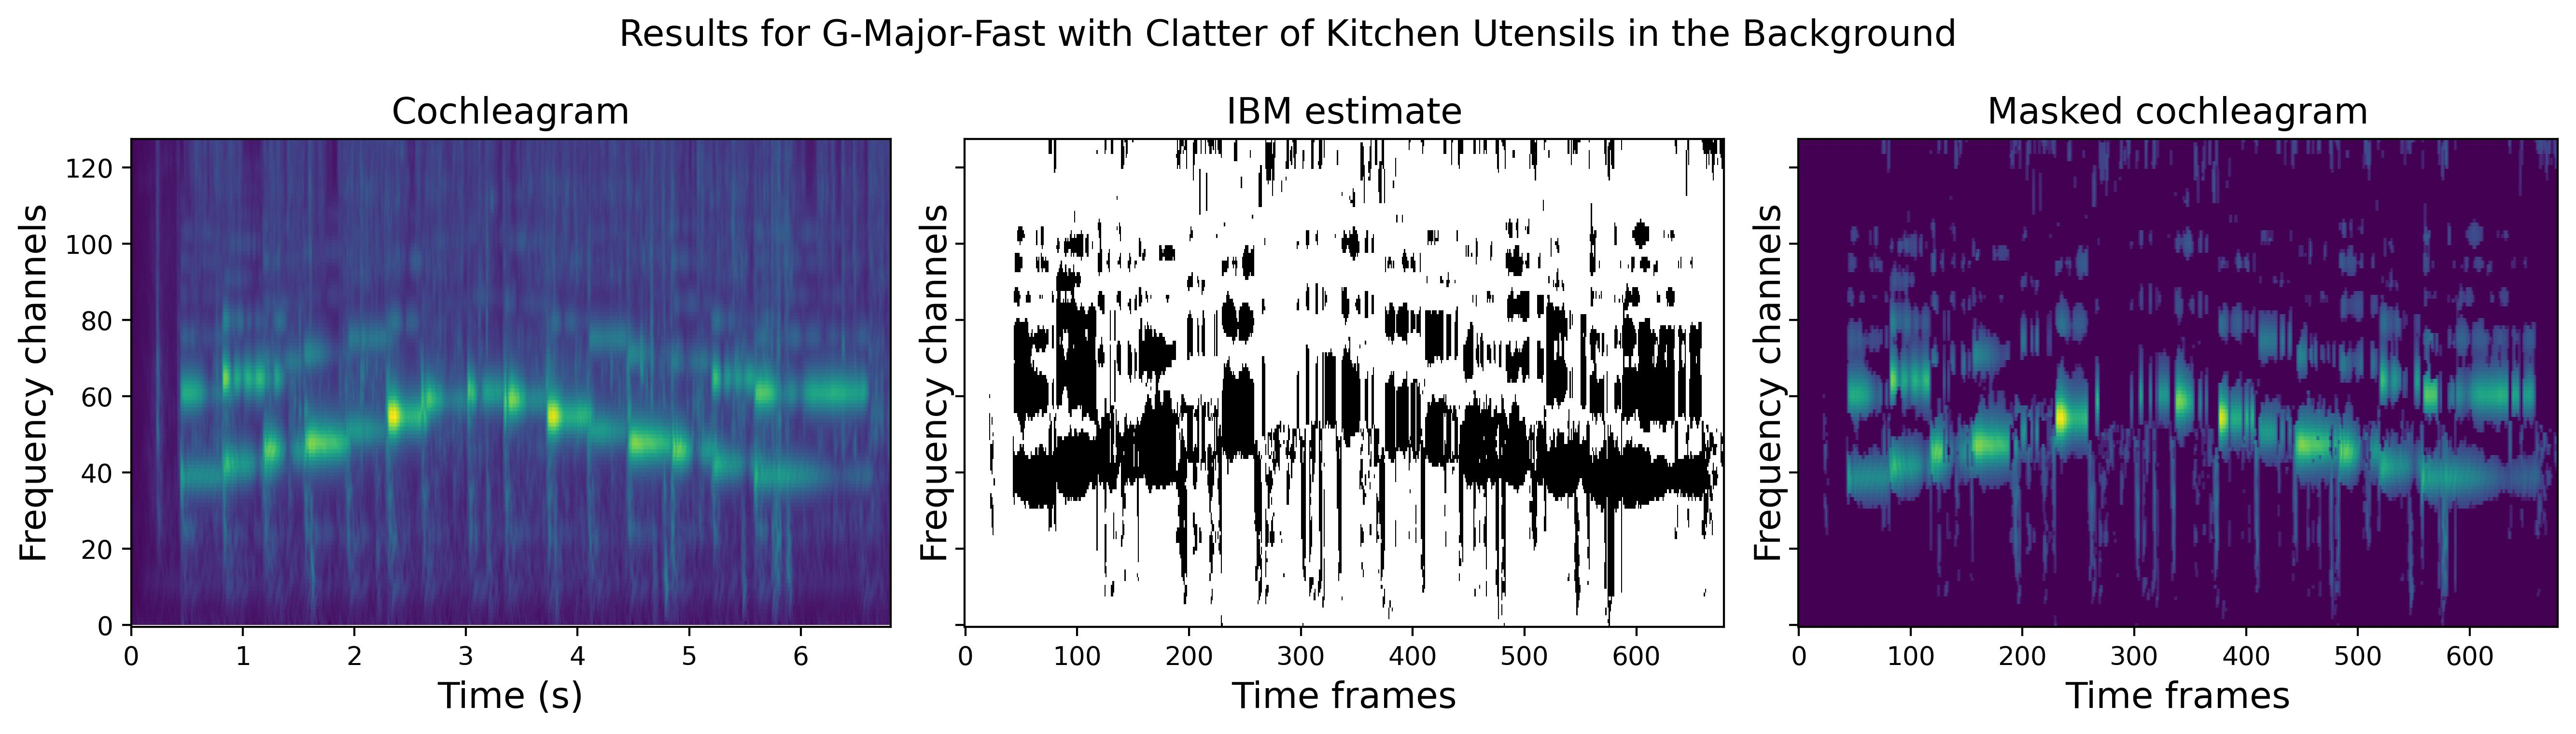
\includegraphics[width=\textwidth]{include/experiments_G-major-fast_BG6.jpg}
	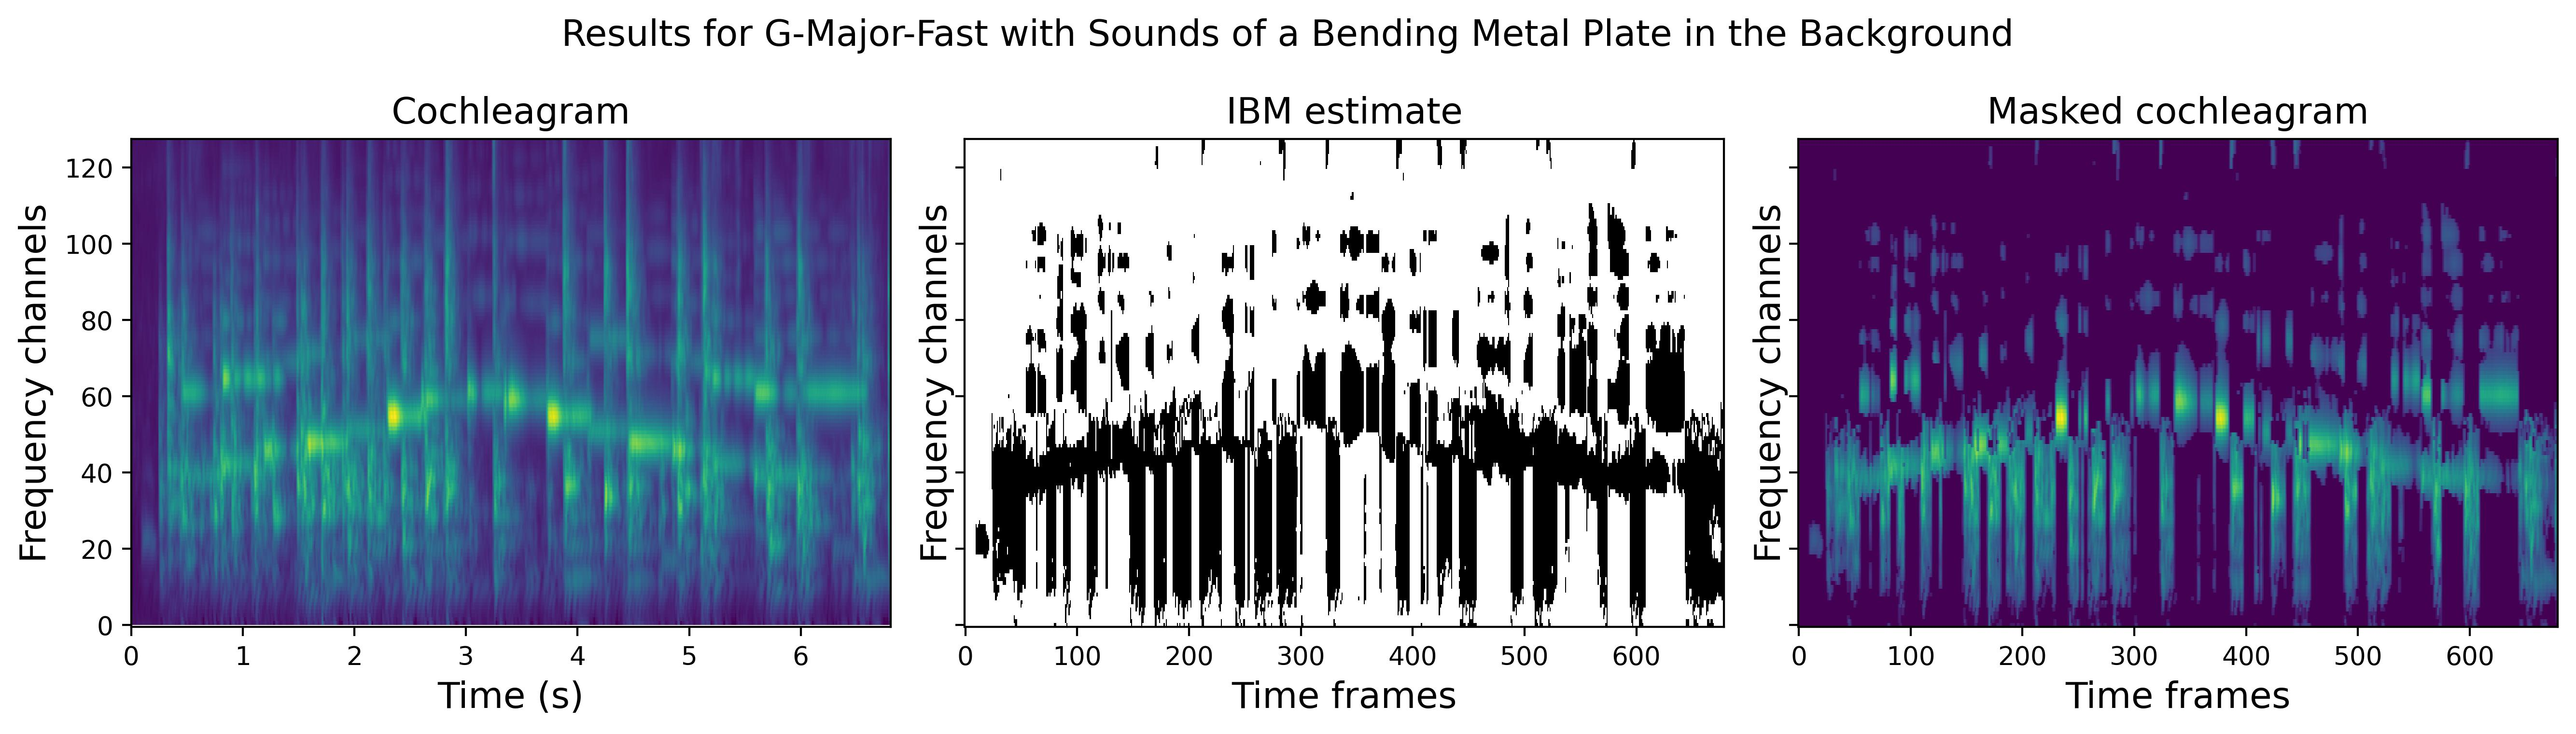
\includegraphics[width=\textwidth]{include/experiments_G-major-fast_BG17.jpg}
	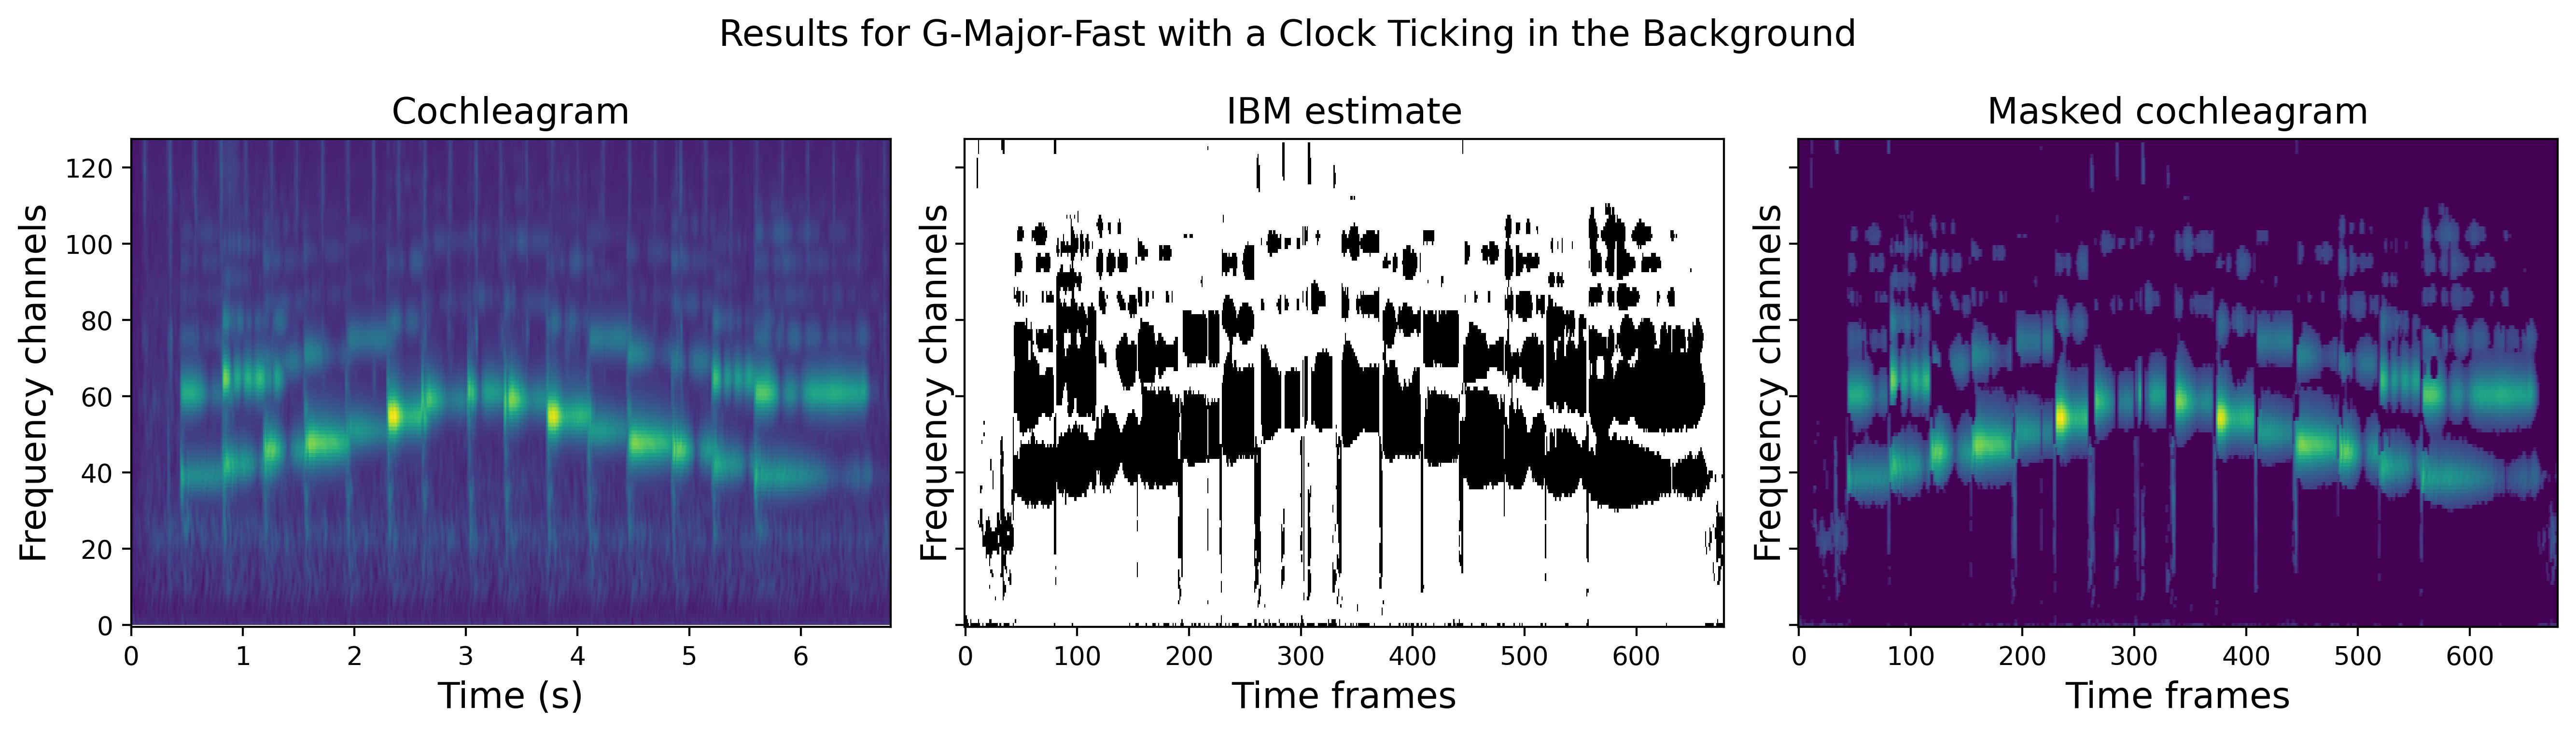
\includegraphics[width=\textwidth]{include/experiments_G-major-fast_BG27.jpg}
	\caption[Results of experiments with other background sounds]{Results of the experiments with G-major scale mixed with other prerecorded sounds in the background. In each row, the first image is a cochleagram of the input sound, the second is the estimated IBM, and the third is the masked cochleagram.}
	\label{img:other_backgrounds_experiments}
\end{figure}

\section{Experiments with Other Backgrounds}

Besides the white noise, other sounds were used in the background too. Among those were various rattling, clanging, ringing or grinding sounds, clatter of kitchen utensils, sounds of rustling paper or a plastic candy wrapper, ticks of a clock, clicks of a computer mouse, and so on. Mainly, these sounds were not harmonic, and therefore did not evoke a perception of pitch. All of them may be found on the attached medium.\\

For the demonstration of these experiments, the noise level parameter was chosen dynami\-cally to better adapt to varying input sound levels and nature of the sounds. Otherwise, the experiments were similar to the ones for white noise levels, and are shown on figure \ref{img:other_backgrounds_experiments}. On the figure, each row represents the results of processing the G-major scale played fast with different background sounds: the first and the second are rustlings of paper and a plastic candy wrapper respectively, the third one is clatter of kitchen utensils, the fourth is a sound of a bending metal plate, and the last one is a sound of a ticking clock.\\

The most interesting results can be seen in the fourth and fifth rows. For the bending metal plate case, the background interference can be well seen on the cochleagram in lower frequency channels. This type of background may be considered harmonic (at least to some extent), and thus some kind of polyphony was created, where the metal plate sounds are heard simultaneously with the piano sounds. Being built to separate only monophonic inputs, the system was not able to process this mixture well enough.\\

The fifth row, in turn, is interesting due to the noise level argument for the clock ticks in the background. In this case, the amplitude was multiplied by a factor of 15.0 (!), however the outcomes don't seem too much affected. This may be explained by the nature of the clock ticking sounds -- they are not harmonic and don't have pitch. All the mixtures for these experiments for different noise level values may be found on the enclosed medium (appendix \ref{chapter:medium}).

\section{Experiments with a Simple Classifier}

The next set of experiments was meant to test the implemented CASA system in connection with a simple classifier. The main thought behind it was to practically prove that CASA processing brings non-zero improvements to the model's accuracy scores and makes the training easier, when the predictions should be made for noisy data. This way, it can be proven that CASA systems may become a good front-end for further applications. For this purpose, the decision tree classifier implementation was chosen from the \textit{scikit-learn} \cite{scikit-learn} package, because of their simplicity and absence of additional required data preparations.\\

The model was trained on two experimental sets of data computed from the dataset described in chapter \ref{section:experiments_dataset}. The first set consisted of unmasked cochleagrams, and the second of masked ones. The cochleagrams were computed for clean input signals, signals with random amounts of added white noise, and signals for sounds with other artificially added backgrounds. The labels for the samples were numerical representations of their corresponding input sounds. The numbers of samples in each group were also chosen experimentally, being one sample for each clean input signal, two samples per input signal with random white noise levels, and two samples per input signal with other random backgrounds with random amplitudes in the $[0; 1]$ range. The argumentation behind this ratio is simple -- the model was going to make predictions primarily for sounds with noisy backgrounds, thus it was trained on high amounts of these, but not left without an ability to recognize the clean ones.\\

Before the training, 40\,\% of the samples were reserved for model validation, because the hyperparameters for the model were chosen in a more simple manner (iteratively). The implementation, of course, saved space for improvement, as well as it allowed to manually override the hyperparameters. Using the best hyperparameters, the model was trained and tested on the two above-mentioned datasets. For testing, sets of 100 samples produced from random input sounds with random backgrounds of random amplitudes were used. The results were more or less expected: the model trained on unmasked cochleagrams had 40--60\,\% accuracy when tested on unmasked cochleagrams, and 50--70\,\% on masked ones. On the other hand, when the model was initially trained on masked data, the accuracy difference was greater: 10--20\,\% for unmasked samples, and 70--90\,\% for the masked ones.

\section{Other Experiments}

As a possibility for deeper research, the implemented system allows to alter other input parameters of its algorithms. For example, different numbers of filters in the gammatone filterbank, their minimum and maximum center frequencies, or parameters of sampling windows might be tested at the peripheral analysis stage. Consequently, the number of autocorrelation lags or harmonics being searched in the summary autocorrelation might be varied at the feature extraction stage. Finally, for the segmentation-and-grouping stage, different numerical thresholds might be chosen for the computes masks. The attached notebook with experiments provides examples of experimenting with the number of searched harmonics. There, some more limitations of the implemented system may be seen.

\section{Chapter Summary}

The experiments chapter firstly reviewed the input dataset for the system described in chapter \ref{chapter:implementation}, and then listed and discussed four sets of experiments, along with their results. Experiments with white noise levels have proven that the implemented system is able to separate input sounds from white noise to some extent. Experiments with other prerecorded backgrounds have shown that the system is most successful when these sounds are not harmonic and don't evoke a perception of pitch. Experiments in connection with a simple classifier have proven that CASA processing may become a good front-end for further applications. And finally, other experiments have shown other limitations of the system and emphasized possible ways of improvement.
